\begin{wrapfigure}{r}{0pt}
  \centering
  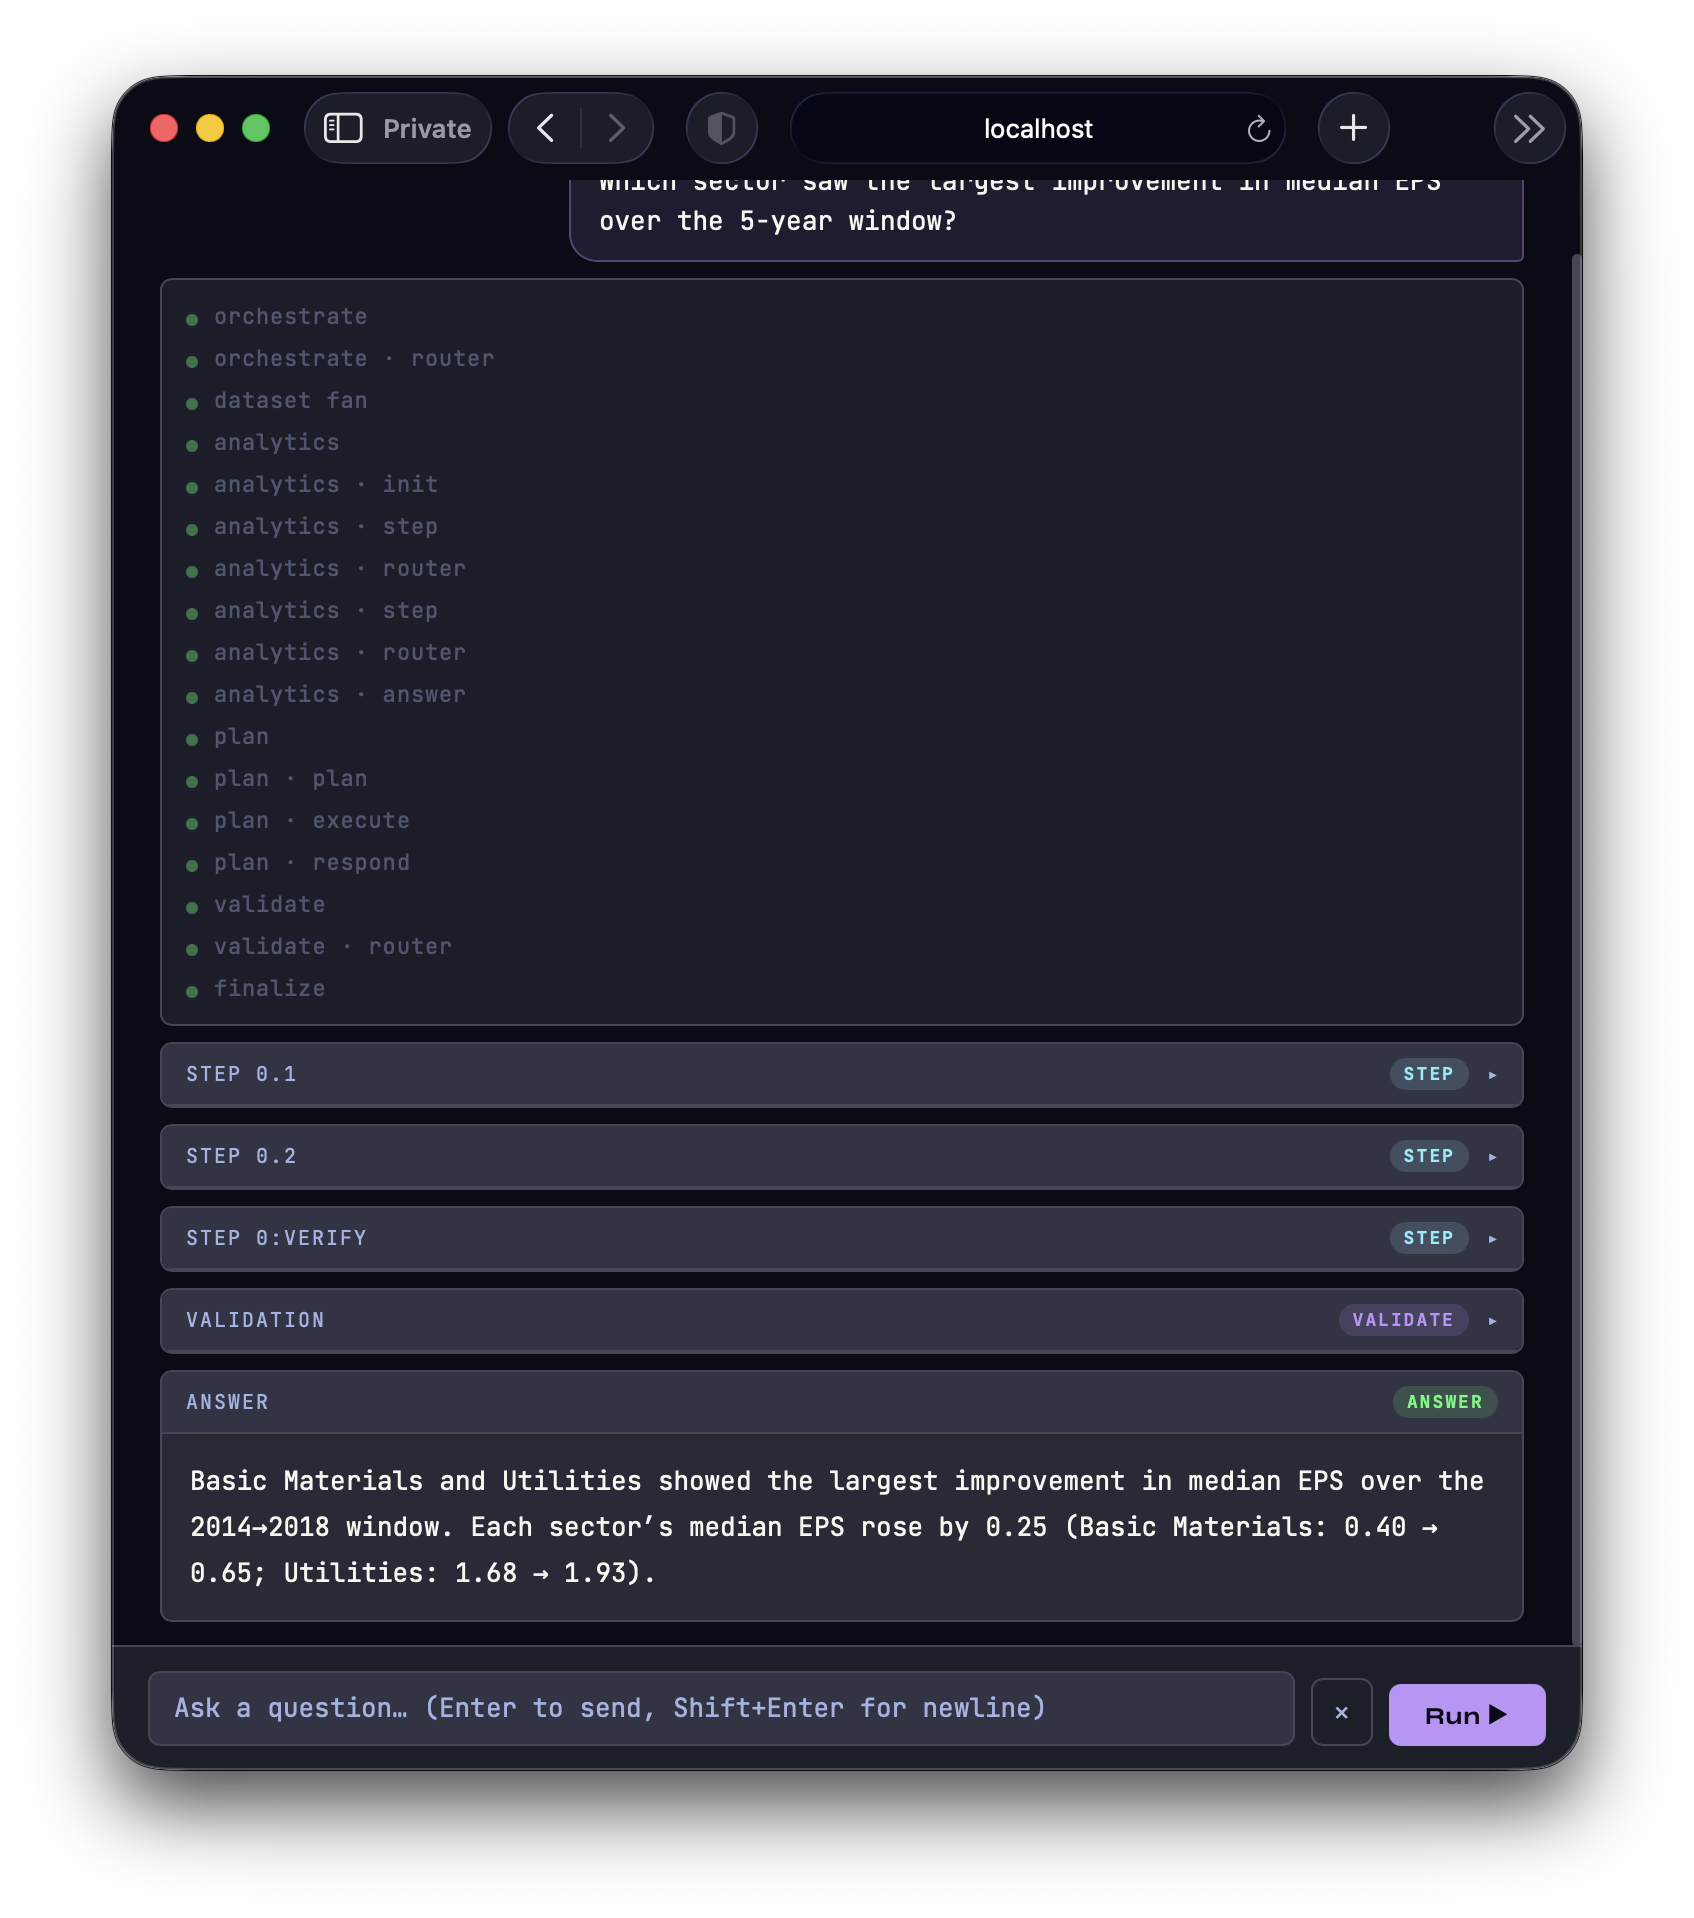
\includegraphics[width=0.4\textwidth]{graphics/ui-which-sector-saw-the-largest-improvement-in-median-eps-over-the-5-year-window.png}
  \caption{UI Screenshot}
\end{wrapfigure}

The agent answers the question by comparing sector-level median earnings per share (EPS) between the beginning and end of the five-year period. Rather than analyzing every intermediate year, it focuses on the net change from 2014 to 2018 and systematically computes the sector-level improvement.

\subsect{Understanding the Analytical Objective}

The agent first interprets the task as a comparison problem. It identifies that the required metric is the change in median EPS for each sector over the five-year window. To answer the question, it plans to:

\begin{itemize}
  \item Compute the median EPS for every sector in 2014.
  \item Compute the median EPS for every sector in 2018.
  \item Compare the two medians by sector.
  \item Identify the sector or sectors with the largest positive change.
\end{itemize}

The agent explicitly defines the improvement metric as:

\[
  \text{Improvement} = \text{Median EPS}_{2018} - \text{Median EPS}_{2014}.
\]

\subsect{Loading and Aggregating the Yearly Data}

Next, the agent loads the financial datasets corresponding to 2014 and 2018. For each dataset, it groups observations by the \texttt{Sector} field and computes the median value of \texttt{EPS}.

This aggregation step transforms thousands of company-level observations into a compact sector-level summary. The resulting outputs are two tables:

\begin{itemize}
  \item Sector median EPS in 2014.
  \item Sector median EPS in 2018.
\end{itemize}

Using medians reduces the influence of extreme EPS values and provides a robust measure of sector performance.

\subsect{Aligning Sector Summaries and Computing Changes}

After obtaining the sector medians for both years, the agent aligns the two summaries by sector and constructs a combined table containing:

\begin{itemize}
  \item Median EPS in 2014.
  \item Median EPS in 2018.
  \item The difference between the two values.
\end{itemize}

The agent also accounts for the possibility that a sector may be missing from one of the years. Any sector lacking a valid median in either year is excluded from the comparison so that the computed change remains meaningful.

\subsect{Identifying the Maximum Improvement}

With the differences calculated, the agent searches for the largest value of the improvement metric. It sorts or scans the sector-level differences and determines the maximum observed increase.

The computed changes reveal that:

\begin{itemize}
  \item Basic Materials improved from 0.40 to 0.65.
  \item Utilities improved from 1.68 to 1.93.
\end{itemize}

Both sectors experienced an increase of:

\[
  0.25 = \text{Median EPS}_{2018} - \text{Median EPS}_{2014}.
\]

\subsect{Handling Ties and Producing the Final Result}

The agent does not assume that only one sector can achieve the maximum improvement. After finding the largest increase, it checks whether multiple sectors share the same value.

This tie-handling step reveals that two sectors achieve the maximum improvement. The agent therefore returns both sectors rather than arbitrarily selecting one.

The final conclusion is that \textbf{Basic Materials} and \textbf{Utilities} tied for the largest improvement in median EPS between 2014 and 2018, with each sector increasing by \textbf{0.25}.